\begin{name}
	{\tenchude}
	{TOÁN 11}
	{LỚP TOÁN THẦY PHÁT}
	{Thời gian: 90 phút - Không kể thời gian phát đề}
\end{name}
\setcounter{ex}{0}\setcounter{bt}{0}
\TN
\Opensolutionfile{ans}[ans/ansDe3-TN1]
\begin{ex}%[Dự án đề kiểm tra Toán 11 HKII NH23-24- Đoàn Minh Tâm]%[1H8H4-3]
Cho hình chóp tứ giác đều $ S.ABCD$ có $ AB=2a$, $ SA=a\sqrt 5 $. Góc giữa hai mặt phẳng $ (SBC)$ và $ (ABCD)$ bằng
\choice
{$30^0$}
{\True $60^0$}
{$45^0$}
{$90^0$}
\loigiai{
\immini{
Gọi $O$ là giao điểm của $AC$ và $BD$, $M$ là trung điểm $BC$.\\
Do $OBC$ là tam giác cân tại $O$ nên $OM\perp BC$.\\
Hơn nữa $SBC$ là tam giác cân tại $S$ nên $SM \perp BC$.\\
$\heva{&OM \perp BC \\&SM \perp BC \\&(SBC)\cap (ABCD)=BC}$\\
$\Rightarrow ((SBC),(ABCD))=(OM,SO)=\widehat{SMO}$.
}{
\begin{tikzpicture}[line join=round,line cap=round,line width=.6pt,font=\footnotesize,scale=1]
\coordinate[label=below left:$B$] (B) at (0,0);
\coordinate[label=above right:$A$] (A) at (1,1.2);
\coordinate[label=below right:$C$] (C) at (4,0);
\coordinate[label=above right:$D$] (D) at ($(C)-(B)+(A)$);
\coordinate[label=below right:$O$] (O) at ($(A)!.5!(C)$);
\coordinate[label=above left:$S$] (S) at ($(O)+(90:5)$);
\coordinate[label=below:$M$] (M) at ($(B)!.5!(C)$);
\draw (B)--(C)--(D)--(S)--cycle (S)--(C) (S)--(M);
\draw[dashed] (C)--(A)--(D)--(B) (O)--(S)--(A)--(B) (O)--(M);
\newcommand{\gocv}[4][black]{\draw[#1] ($(#3)!5pt!(#2)$)--($(#3)!2!($($(#3)!5pt!(#2)$)!.5!($(#3)!5pt!(#4)$)$)$)--($(#3)!5pt!(#4)$);}
\gocv{S}{M}{B}
\gocv{O}{M}{C}
\fill (A)circle(1.5pt) (B)circle(1.5pt) (C)circle(1.5pt) (D)circle(1.5pt) (S)circle(1.5pt) (O)circle(1.5pt) (M)circle(1.5pt);
\draw pic[draw,angle radius=3mm] {angle = O--M--S}; % Vẽ góc BAC
\end{tikzpicture}
}
\noindent Ta có $OM=\dfrac{AB}{2}=\dfrac{2a}{2}=a$ (do $OM$ là đường trung bình $\triangle ABC$).\\
$AO=\dfrac{AC}{2}=\dfrac{AB\sqrt{2}}{2}=a\sqrt{2}$.\\
Khi đó $SO=\sqrt{SA^2-AO^2}=\sqrt{(a\sqrt{5})^2-(a\sqrt{2})^2}=a\sqrt{3}.$\\
Nên $\tan {SMO}=\dfrac{a\sqrt{3}}{a}=\sqrt{3}$.\\
Vậy $\widehat{SMO}=60^\circ$.
}
\end{ex}

\begin{ex}%[BG - 10-11 New - 4in1, Phan Anh]%[1H8H4-2]
Cho hình chóp $S.ABCD$ có đáy $ABCD$ là hình vuông cạnh $a$. Gọi $M, N$ lần lượt là trung điểm của các cạnh $AD$ và $CD$. Biết $(SAN) \perp(ABCD)$ và $(SBM) \perp(ABCD)$. Chọn khẳng định đúng.
\choice
{$ (SAM) \perp(SBN)$}
{$ (SAB) \perp(SMN)$}
{\True $ (SAN) \perp(SBM)$}
{$ (SCD) \perp(SMN)$}
\loigiai{
\immini
{
Trong $(ABCD)$ ta có AN $\cap BM=H \Rightarrow SH=(SAN) \cap(SBM)$.\\
Theo giả thiết, ta có $(SAN) \perp(ABCD)$ và $(SBM) \perp(ABCD)$
$\Rightarrow SH \perp(ABCD) \Rightarrow SH \perp BM$ \quad(1).\\
Mặt khác $\triangle ABM=\triangle DAN \Rightarrow \widehat{ABH}=\widehat{MAH}$
$\Rightarrow \widehat{ABH}+\widehat{BAH}=\widehat{MAH}+\widehat{BAH}=90^{\circ}$\\
$\Rightarrow AN \perp BM$ \quad(2).\\
Từ (1) và (2) $\Rightarrow BM \perp(SAN)$ mà $BM \subset(SBM) \Rightarrow(SAN) \perp(SBM)$.
}
{	\begin{tikzpicture}[scale=0.7, font=\footnotesize, line join=round, line cap=round, >=stealth]
\coordinate (D)at (0,0);
\coordinate (A)at (-3,-2);
\coordinate (C) at (5,0);
\coordinate (B) at ($(A)-(D)+(C)$);
\coordinate (M) at ($(D)!.5!(A)$);
\coordinate (N) at ($(D)!.5!(C)$);
\path
(intersection of B--M and A--N) coordinate (H);
\coordinate (S) at ($(H)+(90:5)$);
\foreach \x/\g in {A/160,B/-20,C/0,D/180,S/90,M/170,N/90,H/-100} \fill (\x) circle (1pt) +(\g:3mm) node{$\x$};
\draw (S)--(B)--(C)--(S)--(A)--(B)--(S);
\draw[dashed] (S)--(D)--(A) (C)--(D) (A)--(N)--(S) (B)--(M)--(S)--(H) ;
\foreach \x in {A,B,C,D,S,M,N,H}	\fill (\x)circle(1.5pt);
\end{tikzpicture}
}
}

\end{ex}

\begin{ex}%[1D6N3-1]
Tập giá trị của hàm số $y=\mathrm{e}^{-2x+4}$ là
\choice
{\True$(0;+\infty)$}
{$[0;+\infty)$}
{$\mathbb{R}\setminus\{0\}$}
{$\mathbb{R}$}
\loigiai{
Vì $\mathrm{e}^{-2x+4}>0\ \forall x\in\mathbb{R}$ nên tập giá trị của hàm số là $(0;+\infty)$.
}
\end{ex}

\begin{ex}%[1H8N6-2]ID%[Dự án đề kiểm tra Toán 11 GHKI NH23-24- Phan Trung Hiếu]%[THPT Nguyễn Hữu Huân- Tp HCM]
Cho hình chóp $S.ABCD$ có đáy $ABCD$ là hình chữ nhật với $SA\perp(ABCD)$. Góc giữa hai mặt phẳng $(SBC)$ và $(ABCD)$ là
\choice
{$\widehat{SCA}$}
{\True $\widehat{SBA}$}
{$\widehat{SDA}$}
{$\widehat{SAB}$}
\loigiai{
Ta có $\heva{&(SBC)\cap(ABCD)=BC\\&AB\perp BC\\&SB\perp BC\, (BC\perp(SAB))}$\\
$\Rightarrow((SBC),(ABCD))=\widehat{SBA}$.
}
\end{ex}

\begin{ex}%[1D6N2-2]
Nếu $\log 4=a$ thì $\dfrac{1}{\log_{256}100}$ bằng
\choice
{$a^4$}
{$\dfrac{a}{8}$}
{\True $ 2a$}
{$ 16a$}
\loigiai{
Ta có $\dfrac{1}{\log_{256}100}=\log_{100}256=\log_{10^2}4^4=\dfrac{4}{2}\log{4}=2a$.}
\end{ex}

\begin{ex}%[1H8H2-2]
\immini{
Cho hình chóp $S.ABCD$ như hình bên. Có đáy $ABCD$ là hình chữ nhật. $SA = SC$ và $SB = SD$. Khẳng định nào sau đây là đúng?
}{
\begin{tikzpicture}[scale=0.8, font=\footnotesize,line join=round, line cap=round, >=stealth]
\path
(0,0) coordinate (A)
++(-140:2) coordinate (B)
++(0:3.5) coordinate (C)
($(A)+(C)-(B)$) coordinate (D)
($(A)!1/2!(C)$) coordinate (O)
($(O)+(0,3.5)$) coordinate (S)
;
\foreach \i in{B,C,D}{\draw (S)--(\i);};
\draw (B)--(C)--(D);
\draw[dashed] (S)--(A)--(B) (C)--(A)--(D)--(B) (S)--(O);
\foreach \i/\g in {A/-90,B/-90,C/-90,D/-90,O/-90,S/90}
\fill[black] (\i) circle(1pt)+(\g:3mm)node[scale=1]{$\i$};
\end{tikzpicture}
}
\choice
{$SO \perp (SAB)$}
{$OC \perp (SBD)$}
{\True $SO \perp (ABCD)$}
{$AB \perp (SAB)$}
\loigiai{
Ta có $SA = SC$ nên $\triangle SAC$ cân tại $S$. Suy ra $SO \perp AC$.\\
Và $SB = SD$ nên $\triangle SBD$ cân tại $S$. Suy ra $SO \perp BD$.\\
Tóm lại $\heva{&SO \perp AC,\, AC \subset (ABCD)\\&SO \perp BD,\, BD \subset (ABCD)\\&AC \cap BD = O} \Rightarrow SO \perp (ABCD)$.
}
\end{ex}

\begin{ex}%[1H8N1-1]
Trong các mệnh đề sau, mệnh đề nào đúng?
\choice
{\True Góc giữa hai đường thẳng $a$ và $b$ bằng góc giữa hai đường thẳng $a$ và $c$ khi $b$ song song hoặc trùng với đường thẳng $c$}
{Góc giữa hai đường thẳng là góc nhọn}
{Góc giữa hai đường thẳng $a$ và $b$ bằng góc giữa hai đường thẳng $a$ và $c$ thì $b$ song song với $c$}
{Góc giữa hai đường thẳng bằng góc giữa hai véc-tơ chỉ phương của hai đường thẳng đó}
\loigiai{
Góc giữa hai đường thẳng $a$ và $b$ bằng góc giữa hai đường thẳng $a$ và $c$ khi $b$ song song hoặc trùng với đường thẳng $c$.
}
\end{ex}

\begin{ex}%[1D6N1-2]%[Dự án đề kiểm tra Toán 11 HKII NH23-24- PHẠM CHÍ DŨNG]%[THPT HÙNG VƯƠNG TPHCM]
Cho $a$ là số thực dương tùy ý và $m$, $n$ là các số thực. Đẳng thức nào sau đây là \textbf{đúng}?
\choice
{$a^m \cdot a ^n = a^{mn}$}
{\True $\left(a^m\right)^n=\left(a^n\right)^m$}
{$a^m+a^n=a^{m+n}$}
{$\dfrac{a^m}{a^n}=a^{\frac{m}{n}}$}
\loigiai{
Theo công thức, ta có $\left(a^m\right)^n=\left(a^n\right)^m=a^{mn}$.
}
\end{ex}

\begin{ex}%[1H8N4-1]
Trong các khẳng định sau về lăng trụ đều, khẳng định nào \textbf{sai}?
\choice
{Đáy là đa giác đều}
{Các mặt bên là những hình chữ nhật nằm trong mặt phẳng vuông góc với đáy}
{Các cạnh bên là những đường cao}
{\True Các mặt bên là những hình vuông}
\loigiai{
\begin{itemize}
\item Khẳng định \lq\lq  Đáy là đa giác đều\rq\rq\, là đúng vì lăng trụ đều nên các cạnh bằng nhau. Do đó đáy là đa giác đều.
\item Khẳng định \lq\lq  Các mặt bên là những hình chữ nhật nằm trong mặt phẳng vuông góc với đáy\rq\rq\, là đúng vì lăng trụ đều là lăng trụ đứng nên các mặt bên vuông góc với đáy.
\item Khẳng định \lq\lq  Các cạnh bên là những đường cao\rq\rq\, là đúng Vì lăng trụ đều là lăng trụ đứng nên các cạnh bên vuông góc với đáy.
\item Khẳng định \lq\lq  Các mặt bên là những hình vuông\rq\rq\, là sai vì lăng trụ đều là lăng trụ đứng nên các cạnh bên bằng nhau và cùng vuông góc với đáy. Do đó các mặt bên là những hình vuông.
\end{itemize}
}
\end{ex}

\begin{ex}%[1H8N6-1]ID%[Dự án đề kiểm tra Toán 11 GHKI NH23-24- Phan Trung Hiếu]%[THPT Nguyễn Hữu Huân- Tp HCM]
Cho hình chóp $S.ABC$ có $SA\perp(ABC)$ và $AB\perp BC$. Góc giữa đường thẳng $SC$ và mặt phẳng $(ABC)$ là góc nào sau đây?
\choice
{Góc $\widehat{CSB}$}
{Góc $\widehat{SCB}$}
{\True Góc $\widehat{SCA}$}
{Góc $\widehat{CSA}$}
\loigiai{
Ta có $\heva{&SC\cap(ABC)\\&SA\perp(ABC)}\Rightarrow(SC,(ABC))=\widehat{SCA}$.
}
\end{ex}

\begin{ex}%[1H8H6-2]%[Dự án đề kiểm tra Toán 11 HKII NH23-24-  Pham Quoc Toan]%[THPT TRUNGHOCTHUCHANH- Tp HCM]
Cho hình chóp $S. ABCD$ có đáy $ABCD$ là hình vuông cạnh $a$, $SA$ vuông góc với mặt phẳng $\left(ABCD \right)$ và $SA = \dfrac{a \sqrt{2}}{2}$. Khi đó, số đo góc nhị diện $[S, BD, A]$ bằng
\choice
{$90^{\circ}$}
{$60^{\circ}$}
{$30^{\circ}$}
{\True $45^{\circ}$}
\loigiai{
\begin{center}
\begin{tikzpicture}[scale=0.8, font=\footnotesize, line join=round, line cap=round, >=stealth]
\coordinate (A) at (3,3);
\coordinate (B) at (7,3);
\coordinate (C) at (4,0);
\coordinate (D) at (0,0);
\coordinate (S) at (3,6);
\coordinate (O) at (3.5,1.5);
\draw (S)--(B) (B)--(C) (C)--(D)--(S)--(C);
\draw[dashed] (A)--(B) (A)--(S) (A)--(D) (A) -- (C) (B) -- (D) (S) -- (O);
\foreach \x/\g in {S/90,A/180,B/0,C/0,D/180, O/-90} \fill (\x) circle (1pt) +(\g:3mm) node{$\x$};
\foreach \a/\b/\c in {S/A/B,S/A/D, S/O/B, A/O/D}{\draw pic[draw,angle radius=2mm] {right angle = \a--\b--\c};}
\end{tikzpicture}
\end{center}
Ta có $\heva{& \left(SBD \right) \cap \left(ABD \right) = BD \\ & AO \perp BD \\ & SO \perp BD} \Rightarrow [S, BD, A] = \widehat{SOA}$. \\
Do $AC = \sqrt{AB^2 + BC^2} = a \sqrt{2} \Rightarrow AO = \dfrac{a \sqrt{2}}{2}$. \\
Tam giác vuông $SAO$ có $SA= AO$ nên là tam giác vuông cân. Vậy $\widehat{SOA} = 45^{\circ}$.
}
\end{ex}

\begin{ex}%[1H8N2-1]
Trong không gian mặt phẳng $(P)$ và đường thẳng $d$ không vuông góc với mặt phẳng $(P)$. Hãy chọn mệnh đề đúng trong các mệnh đề dưới đây.
\choice
{Tồn tại duy nhất một mặt phẳng $(Q)$ chứa đường thẳng $d$ và $(Q)$ song song với $(P)$}
{Không tồn tại mặt phẳng $(Q)$ chứa đường thẳng $d$ và $(Q)$ song song với $(P)$}
{\True Tồn tại duy nhất một mặt phẳng $(Q)$ chứa đường thẳng $d$ và $(Q)$ vuông góc với $(P)$}
{Tồn tại duy nhất một đường thẳng $\Delta$ nằm trên mặt phẳng $(P)$ và $\Delta$ vuông góc với $d$}
\loigiai{Tồn tại duy nhất một mặt phẳng $(Q)$ chứa đường thẳng $d$ và $(Q)$ vuông góc với $(P)$.}
\end{ex}
\Closesolutionfile{ans}

\TNTF
\Opensolutionfile{ans}[ans/ansDe3-TN2]
\begin{ex} 	%[1D6H2-3]
Trong các khẳng định sau, khẳng định nào đúng, khẳng định nào sai?
\choiceTF
{ Với $0< a \ne 1, b> 0 $ ta có $a^{\log_{\sqrt{a}}b} = b$}
{\True  Với $0< a \ne 1$ ta có $\log_{a^2}{a^4} = \dfrac{4}{2}$}
{\True Với $0< a \ne 1$ và $\log_4{a} = x, \log_4{b} = y$ ta có $\log_4(a^{4}\sqrt[3]{b^{3}}) = 4x + \dfrac{3}{3}y$}
{Với $0< a \ne 1$ ta có $\log_{\sqrt[3]{a}}{{a}^4} = 7$}
\loigiai{
\begin{itemchoice}
\itemch Ta có \[\log_{\sqrt{a}}b = \dfrac{\log_a{b}}{\log_a{\sqrt{a}}} = 2\log_a{b} = \log_a{b^2}.\] Do đó $a^{\log_{\sqrt{a}}b} = a^{log_a{b^2}} = b^2$
\itemch Ta có \[\log_{a^2}{a^4} = \dfrac{4}{2}\log_a{a} = \dfrac{4}{2}.\]
\itemch Ta có \[\log_4(a^{4}\sqrt[3]{b^{3}}) = 4\log_4a + \dfrac{3}{3}\log_4b = 4x + \dfrac{3}{3}y.\]
\itemch Ta có \[\log_{\sqrt[3]{a}}{{a}^4} =3\cdot 4 \cdot \log_{a}{a} = 12.\]
\end{itemchoice}}

\end{ex}

\begin{ex}%[1H8H6-1]
Cho hình chóp $S.ABC$ có đáy $ABC$ là tam giác đều cạnh $a$. Biết $SA=a\sqrt{2}$ và $SA$ vuông góc với mặt đáy. Gọi $M$ là trung điểm của $BC$ và $H$ là hình chiếu vuông góc của $A$ lên $SM$.
\choiceTF[t]
{\True Đường thẳng $AH$ vuông góc với mặt phẳng $(SBC)$}
{\True Đường thẳng $SH$ là hình chiếu của đường thẳng $SA$ lên mặt phẳng $(SBC)$}
{Độ dài đoạn thẳng $AH$ bằng $\dfrac{6a}{11}$}
{Cosin góc tạo bởi đường thẳng $SA$ và mặt phẳng $(SBC)$ bằng $\dfrac{\sqrt{11}}{33}$}
\loigiai{
\immini{
\begin{itemchoice}
\itemch {\bf{Đúng}}. Vì $ABC$ là tam giác đều nên $BC \perp AM$.\\
Lại có $BC \perp SA$, nên $BC \perp (SAM)\Rightarrow  BC \perp AH$.\\
Mặt khác $AH \perp SM$, do đó $AH \perp (SBC)$.
\itemch {\bf{Đúng}}. Vì $AH \perp (SBC)$ nên hình chiếu của $SA$ lên $(SBC)$ là $SH$.
\itemch {\bf{Sai}}. $AM$ là đường trung tuyến của tam giác đều $ABC$ nên $AM=\dfrac{a\sqrt{3}}{2}$.\\
Tam giác $SAM$ vuông tại $A$, có $AH$ là đường cao nên \[AH=\dfrac{SA\cdot AM}{\sqrt{SA^2+AM^2}}=\dfrac{a\sqrt{2}\cdot \dfrac{a\sqrt{3}}{2}}{\sqrt{2a^2+\dfrac{3a^2}{4}}}=\dfrac{a\sqrt{66}}{11}.\]
\itemch {\bf{Sai}}. Hình chiếu của $SA$ lên $(SBC)$ là $SM$ nên \[\cos\left(SA,(SBC)\right)=\cos(SA,SM)=\cos\widehat{ASM}=\dfrac{SA}{SM}=\dfrac{a\sqrt{2}}{\sqrt{2a^2+\dfrac{3a^2}{4}}}=\dfrac{2\sqrt{22}}{11}.\]
\end{itemchoice}
}
{
\begin{tikzpicture}[scale=1, font=\footnotesize, line join=round, line cap=round, >=stealth]
\def\a{3} \def\b{1.8} \def\h{2.2}
\path
(0:0) coordinate (A)
(0:\a) coordinate (C)
(-60:\b) coordinate (B)
($(A)+(90:\h)$) coordinate (S)
($(B)!1/2!(C)$) coordinate (M)
($(S)!1/2.2!(M)$) coordinate (H)
;
\draw (S)--(A)--(B)--(C)--(S)--(B) (S)--(M);
\draw[dashed] (A)--(C) (M)--(A)--(H);
\foreach \x/\g in {S/90,A/180,B/-90,C/0,M/-45,H/45}
\fill[black] (\x) circle(1pt) ($(\x)+(\g:3mm)$) node{$\x$};
\draw pic[draw,blue,angle radius=2mm] {right angle = A--H--M};
\end{tikzpicture}
}
}
\end{ex}
\Closesolutionfile{ans}

\TNSA
\Opensolutionfile{ans}[ans/ansDe3-TN3]
\begin{ex}%[1D6N3-1]%[TeX hóa đề CK2-form 2025 - đợt 2 - Lê Hữu Kiệt]
	\immini
	{Đồ thị như hình vẽ bên là của hàm số $y=\log_a x$ (với $a>0$). Tính $\log_a 2$ (làm tròn đến hàng phần trăm).
	\shortans{0{,}63}
	}
	{
	\begin{tikzpicture}[font=\footnotesize]
	\draw[-stealth] (-0.5,0)--(3.5,0)node[above]{$x$};
	\draw[-stealth] (0,-1.8)--(0,1.5)node[left]{$y$};
	\draw[smooth] plot [domain=0.2:3.3] (\x,{ln(\x)/ln(3)});
	\draw[dashed] (3,0)--(3,1)--(0,1);
	\draw (0,0)node[below left]{$O$};
	\foreach \x in {(1,0), (3,0), (3,1), (0,1)}{\fill[black] \x circle (1pt);}
	\draw (1,0) node[below]{$1$} (3,0)node[below]{$3$} (0,1)node[left]{$1$};
	\end{tikzpicture}
	}
	\loigiai{
	Đồ thị có hình dáng đồ thị của hàm số lôgarit, đi qua điểm $(3;1)$ nên đây là đồ thị hàm số $y=\log_3 x$.\\
	Do đó $\log_3 2 \approx 0{,}63$.
	}
\end{ex}

\begin{ex}%[1D6H4-4]%[Dự án đề kiểm tra Toán 11 HKII NH23-24, Nhật Thiện]%[THPT Lý Thường Kiệt - TPHCM]
	Tích tất cả các nghiệm của phương trình $100^{x^2-2}=0{,}1^{x^2+1}$ là
	\shortans{$-1$}
	\loigiai{
	Ta có
	\[100^{x^2-2}=0{,}1^{x^2+1}\Leftrightarrow 10^{2(x^2-2)}=10^{-1(x^2+1)}\Leftrightarrow 2x^2-4=-x^2-1\Leftrightarrow 3x^2-3=0\Leftrightarrow \hoac{&x=1\\&x=-1.}\]
	Vậy tích tất cả các nghiệm của phương trình là $-1$.
	}
	\end{ex}

\begin{ex}%[1H8V6-7]
	Half time show của Super Bowl $2023$ thuộc về ngôi sao nhạc pop Rihanna. Màn trình diễn của cô gây ấn tượng mạnh mẽ trên $7$ nền sân khấu lơ lửng ở độ cao từ $4{,}5$ m đến $18$ m. Mỗi nền sân khấu được gắn đèn LED nhấp nháy giống như Rihanna đang biểu diễn trên những đám mây. Để có thể tạo được sân khấu có hiệu ứng tốt mà vẫn đảm bảo an toàn, sân khấu sẽ được kết nối bởi $4$ sợi dây cáp có ròng rọc lên một khung sắt chắc chắn sao cho hình chiếu của ròng rọc luôn nằm ở trung điểm các viền của sân khấu (minh họa như hình vẽ). Khi sân khấu chạm mặt đất, độ cao từ khung sắt đến sân khấu là $25$ m, độ dài dây cáp lúc này được điều chỉnh thành $50$ m. Khi đó góc tạo bởi dây cáp và sân khấu sẽ có giá trị là?\\
	\begin{tabular}{lr}
		%\includegraphics[scale=0.64]{images/Picture1.jpg}
		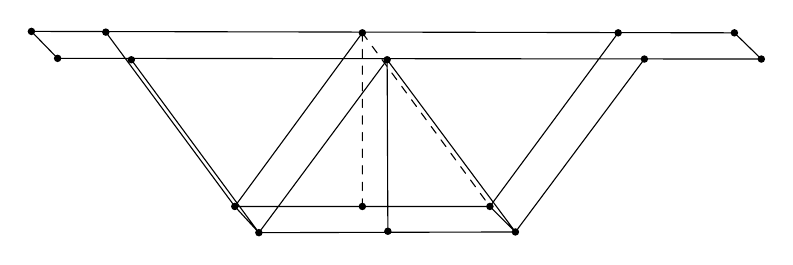
\begin{tikzpicture}[line join=round,line cap=round,>=stealth,font=\footnotesize,scale=.9]
			\path
			(0,0) coordinate (A)
			(0.34,-0.37) coordinate (B)
			(3.6,0) coordinate (D)
			(3.96,-0.36) coordinate (C)
			(1.8,2.45) coordinate (S')
			(2.15,2.07) coordinate (S)
			(1.8,0) coordinate (O')
			(2.16,-0.35) coordinate (O)
			(5.41,2.45) coordinate (I)
			(5.78,2.08) coordinate (J)
			(7.05,2.45) coordinate (K)
			(7.43,2.08) coordinate (L)
			(-1.82,2.46) coordinate (M)
			(-1.46,2.07) coordinate (P)
			(-2.5,2.09) coordinate (Q)
			(-2.87,2.47) coordinate (R)
			;
			\draw (R)--(K)--(L)--(Q)--cycle (A)--(D)--(C)--(B)--cycle (P)--(B)--(S)--(C)--(J) (M)--(A)--(S') (D)--(I) (S)--(O);
			\draw[dashed] (S')--(O') (S')--(D);
			\foreach \x/\g in {A/0,B/0,C/0,D/0,S/0,S'/0,O/0,O'/0,I/0,J/0,K/0,L/0,M/0,P/0,Q/0,R/0}
			\fill[black] 	(\x) circle (1.5pt);
		\end{tikzpicture}
	\end{tabular}
	\shortans[0]{$30$}
	\loigiai{
		Dựa theo hình vẽ và yêu cầu đề bài, ta có khối hình sau\\
		\begin{center}
			\begin{tikzpicture}[line join=round,line cap=round,>=stealth,font=\footnotesize,scale=1]
				\path
				(0,0) coordinate (A)
				(0.34,-0.37) coordinate (B)
				(3.6,0) coordinate (D)
				(3.96,-0.36) coordinate (C)
				(1.8,2.45) coordinate (S')
				(2.15,2.07) coordinate (S)
				(1.8,0) coordinate (O')
				(2.16,-0.35) coordinate (O)
				(5.41,2.45) coordinate (I)
				(5.78,2.08) coordinate (J)
				(7.05,2.45) coordinate (K)
				(7.43,2.08) coordinate (L)
				(-1.82,2.46) coordinate (M)
				(-1.46,2.07) coordinate (P)
				(-2.5,2.09) coordinate (Q)
				(-2.87,2.47) coordinate (R)
				;
				\draw (A)--(D)--(C)--(B)--cycle (S')--(S) (S)--(O) (A)--(S') (B)--(S)--(C);
				\draw[dashed] (S')--(O') (S')--(D);
				\foreach \x/\g in {A/180,B/220,C/0,D/30,S/0,S'/180,O/-90,O'/130}
				\fill[black] 	(\x) circle (1.5pt)
				($(\g:3mm)+(\x)$) node {$\x$}
				;
				\draw pic[draw,angle radius=3mm]{right angle=D--O'--S'};
				\draw pic[draw,angle radius=3mm]{right angle=C--O--S};
			\end{tikzpicture}
		\end{center}
		Với
		$\heva{&SB=S’A=SC=S’D=50 \text{ m}\\ &SO=S’O’=25 \text{ m}.}$\\
		Theo yêu cầu đề bài, chính là đi tìm góc giữa đường thẳng $SB$ và $(ABCD)$.\\
		Ta có Do $O$ là hình chiếu của $S$ lên $(ABCD)$ nên $SO$ vuông với $(ABCD)$.\\
		Mà $B$ thuộc $(ABCD)$.\\
		Nên $\left(\widehat{SB,(ABCD)}\right)=(\widehat{SB,SO})=\widehat{SBO}$.\\
		Xét tam giác $SBO$ vuông tại $O$, theo lượng giác trong tam giác vuông, ta có\\
		$\sin\widehat{SBO}=\dfrac{SO}{SB}=\dfrac{25}{30}=\dfrac{1}{2} \Rightarrow \widehat{SBO}=30^\circ$.
	}
\end{ex}

\begin{ex}%[1D6V3-5]
Anh Toàn được tuyển dụng vào một công ty đầu năm $2013$. Công ty trả lương cho anh theo nguyên tắc: Lương khởi điểm anh nhận là $6$ triệu đồng/ tháng và cứ sau $3$ năm công ty lại tăng lương cho anh thêm $25\%$ số lương đang hưởng. Hiện nay (năm $2024$) anh đang được hưởng lương là bao nhiêu triệu đồng một tháng? (Kết quả làm tròn đến hàng phần mười).
%\par
\shortans{$11{,}7$}
\loigiai{
Tính từ năm $2013$ đến năm $2024$, anh Toàn đã được $3$ lần tăng lương.\\
Lương của anh Toàn sau lần tăng đầu tiên là $L_1=6\cdot 1{,}25$ triệu.\\
Lương của anh Toàn sau lần tăng thứ hai là $L_2=L_1+25\%\cdot L_1=L_1\cdot 1{,}25=6\cdot (1{,}25)^2$ triệu.\\
Lương của anh Toàn sau lần tăng thứ ba là $L_3=L_2+25\cdot \%L_2=6\cdot (1{,}25)^3\approx 11{,}7$ triệu.\\
Vậy lương của anh Toàn hiện đang hưởng là $11{,}7$ triệu mỗi tháng.
}
\end{ex}

\Closesolutionfile{ans}

\TL
\begin{ex}%[1D6H4-4]%[Dự án đề kiểm tra Toán 11 HKII NH23-24- Nguyễn Hoàng Anh]%[THPT Nguyễn Thượng Hiền - Tp HCM]
Giải phương trình $\log_{2}(3x+1)+\log_{2}(x-1)=2$.
\loigiai{
Điều kiện $x>1$.\\
Ta có
\begin{eqnarray*}
&&\log_{2}(3x+1)+\log_{2}(x-1)=2\\
&\Leftrightarrow& \log_{2}[(3x+1)(x-1)]=2\\
&\Leftrightarrow& \log_{2}(3x^2-2x-1)=2\\
&\Leftrightarrow& 3x^2-2x-1=4\\
&\Leftrightarrow& 3x^2-2x-5=0\\
&\Leftrightarrow& \hoac{&x=-1 \hspace{0.2 cm} \text{(loại)}\\&x=\dfrac{5}{3}.}
\end{eqnarray*}
Vậy phương trình có một nghiệm $x=\dfrac{5}{3}$.
}
\end{ex}

\begin{ex}%[1H3G3-2]
	Cho hình lăng trụ đứng $ABC.A'B'C'$ có $AA'=BC=a$, $AC=a\sqrt{3}$ và $\Delta ABC$ vuông tại $B$. Điểm $M$ nằm trên cạnh $AC$ sao cho $AM=\dfrac{1}{3}AC$. Chứng minh rằng $B'M \perp A'C$.
	\loigiai{
		\begin{center}
			\begin{tikzpicture}
			\tkzDefPoints{0/0/A, 4/0/C, 3/-1/B, 0/4/A', 4/4/C', 3/3/B', 1.33/0/M, 1.5/-0.5/N}
			\tkzDrawSegments(A,B B,C A',B' B',C' A',C' A,A' B,B' C,C' A',B B',N)
			\tkzDrawSegments[dashed](A,C A',C B',M M,N)
			\tkzMarkRightAngle(A,B,C)
			\tkzMarkRightAngle(A',A,C)
			\tkzLabelPoints[above](A',B',C')
			\tkzLabelPoints[above left](M)
			\tkzLabelPoints[below](A,B,C, N)
			\end{tikzpicture}
		\end{center}
		Gọi $N$ là trung điểm $AB$.\\
		$\Delta ABC$ vuông tại $B$ nên $AB=\sqrt{AC^2-BC^2}=\sqrt{3a^2-a^2}=a\sqrt{2}$.
		\\ Ta có $\dfrac{BN}{BB'}=\dfrac{\frac{a}{\sqrt{2}}}{a} =\dfrac{1}{\sqrt{2}}$, $\dfrac{BB'}{A'B'} =\dfrac{a}{a\sqrt{2}}=\dfrac{1}{\sqrt{2}}$.
		\\ Ta lại có $\widehat{NBB'} =\widehat{BB'A'}$ (cùng là góc vuông) nên $\Delta NBB' \sim \Delta BB'A'$.
		\\ Suy ra $\widehat{B'NB} =\widehat{A'BB'} \Rightarrow \widehat{B'NB} + \widehat{A'BB'} =\widehat{A'BB'} +\widehat{A'BB'} = 90^\circ$. Vì vậy $B'N \perp A'B$ $(1)$.
		\\ Ta có $\begin{cases}
		BB' \perp  BC \\ BC \perp AB 
		\end{cases} \Rightarrow CB \perp (ABB'A')$ $(2)$.
		\\ Từ $(1),(2)$ theo định lý ba đường vuông góc ta có $B'N \perp A'C$ $(3)$.
		\\ Ta có $\dfrac{AM}{AB} =\dfrac{AC}{3AB}=\dfrac{a\sqrt{3}}{3a\sqrt{2}}=\dfrac{1}{\sqrt{6}}$, $\dfrac{AN}{AC} = \dfrac{AB}{2AC}=\dfrac{a\sqrt{2}}{2a\sqrt{3}} =\dfrac{1}{\sqrt{6}}$. Suy ra $\Delta AMN \sim \Delta ABC$.
		\\ Vì vậy $\widehat{AMN} = \widehat{ABC}$ hay $MN \perp AC$. 
		\\ Mặt khác $(ACC'A) \perp (ABC)$ nên suy ra $MN \perp (ACC'A') \Rightarrow MN \perp A'C$ $(4)$.
		\\ Từ $(3),(4)$ ta suy ra $A'C \perp (B'MN) \Rightarrow A'C \perp B'M$.
	}
\end{ex}

\begin{ex}%[1D6V4-6]
	Năm $2\,022$, một hãng công nghệ có $30$ triệu người dùng phần mềm của họ. Hãng đặt kế hoạch, trong $3$ năm tiếp theo, mỗi năm số lượng người dùng phần mềm tăng $8\%$ so với năm trước và từ năm thứ $4$ trở đi, số lượng người dùng phần mềm sẽ tăng $5\%$ so với năm trước đó. Theo kế hoạch đó, hỏi bắt đầu từ năm nào số lượng người dùng phần mềm của hãng sẽ vượt quá $50$ triệu người?
	% \shortans[oly]{2031}
	\loigiai{
	Số lượng người dùng phần mềm của công ty sau $3$ năm
	\[T_1=30\cdot \left(1+\dfrac{8}{100} \right)^3\approx 37{,}79.\]
	Số lượng người dùng phần mềm của công ty sau $n$ năm tiếp theo \[T_2=37{,}79\cdot \left(1+\dfrac{5}{100} \right)^n.\]
	Để người dùng vượt quá $50$ triệu người thì\\
	\[37{,}79\cdot \left(1+\dfrac{5}{100} \right)^n > 50\Leftrightarrow n > 5.\]
	Mà $n\in \mathbb{N}$ nên $n=6$.\\
	Suy ra cần ít nhất $3+6=9$ năm.\\
	Vậy bắt đầu từ năm $2\,022+9=2\,031$ thì số lượng người dùng phần mềm của hãng sẽ vượt quá $50$ triệu người
	}
	\end{ex}
% \Closesolutionfile{ansbook}
% \HetDe
% \label{De3}
% %
% \cleardoublepage
% \setcounter{page}{1}
% \rfoot{Trang \thepage/\pageref{DA3} - Đáp án trắc nghiệm Mã đề 3}
% \begin{center}
% 	\bfseries ĐÁP ÁN TRẮC NGHIỆM MÃ ĐỀ 3
% \end{center}

% \inputansbox{10}{ans/ansDe3-TN1}
% \inputansbox[3]{2}{ans/ansDe3-TN2}
% \inputansbox{3}{ans/ansDe3-TN3}
% \label{DA3}
%
